%#!platex --src-specials main.tex

\chapter{関連研究}

本章では,本研究に必要な予備知識と関連研究について述べる.

\section{機械受容器}

\subsection{機械受容器とは}
機械受容器とは外部との接触または自己の運動や姿勢の変化によって起こる,圧迫・伸展
などの皮膚,筋,腱,関節の変化を検出する細胞や神経終末といった受容器である.
人の皮膚構造にはメルケル細胞,マイスナー小体,パチニ小体,ルフィニ終末の4種の
機械受容器が存在しており,0$-$数百Hzの時間周波数特性と分布の違いによる
空間周波数特性を持っている\cite{岩村吉晃1984ヒト触覚受容器の構造と特性}.
その4種の機械受容器を図\ref{2-1}に示す.
\begin{figure}[h]
  %\begin{minipage}{0.5\hsize}
    \begin{center}
    \includegraphics[width=10cm]{Corpuscles.eps}
    \caption{機械受容器(\cite{Touch:Iwamura}より改変)}
    \label{2-1}
   \end{center}
   \end{figure}
 %\end{minipage}

\subsection{時間周波数特性}
4つの機械受容器の内,メルケル細胞\ (SA\rm\,I\,),マイスナー小体\
(FA\rm\,I\,),パチニ小体\ (FAI\hspace{-.01em}I)
の3つの時間周波数特性を図\ref{2-2}に示す.
図\ref{2-2}の横軸が周波数,縦軸が振幅閾値を表しており,振幅閾値が小さいほど
応答性能がよいということである.図\ref{2-2}よりメルケル細胞が約\ 5\ Hz,
マイスナー小体が約\ 50\ Hz,パチニ小体が約\ 200\ Hz程度の振動に高い感度を
もつことがわかる.本研究では
このマイスナー小体やパチニ小体などの感覚受容器を主なターゲットとする.
また,このパチニ小体が1章で記した振動方向の判別能力が低い受容器であり,
振動を用いた触覚提示において振動方向が重要視されていない要因の一つである.


 %\begin{minipage}{0.5\hsize}
 \begin{figure}[h]
   \begin{center}
   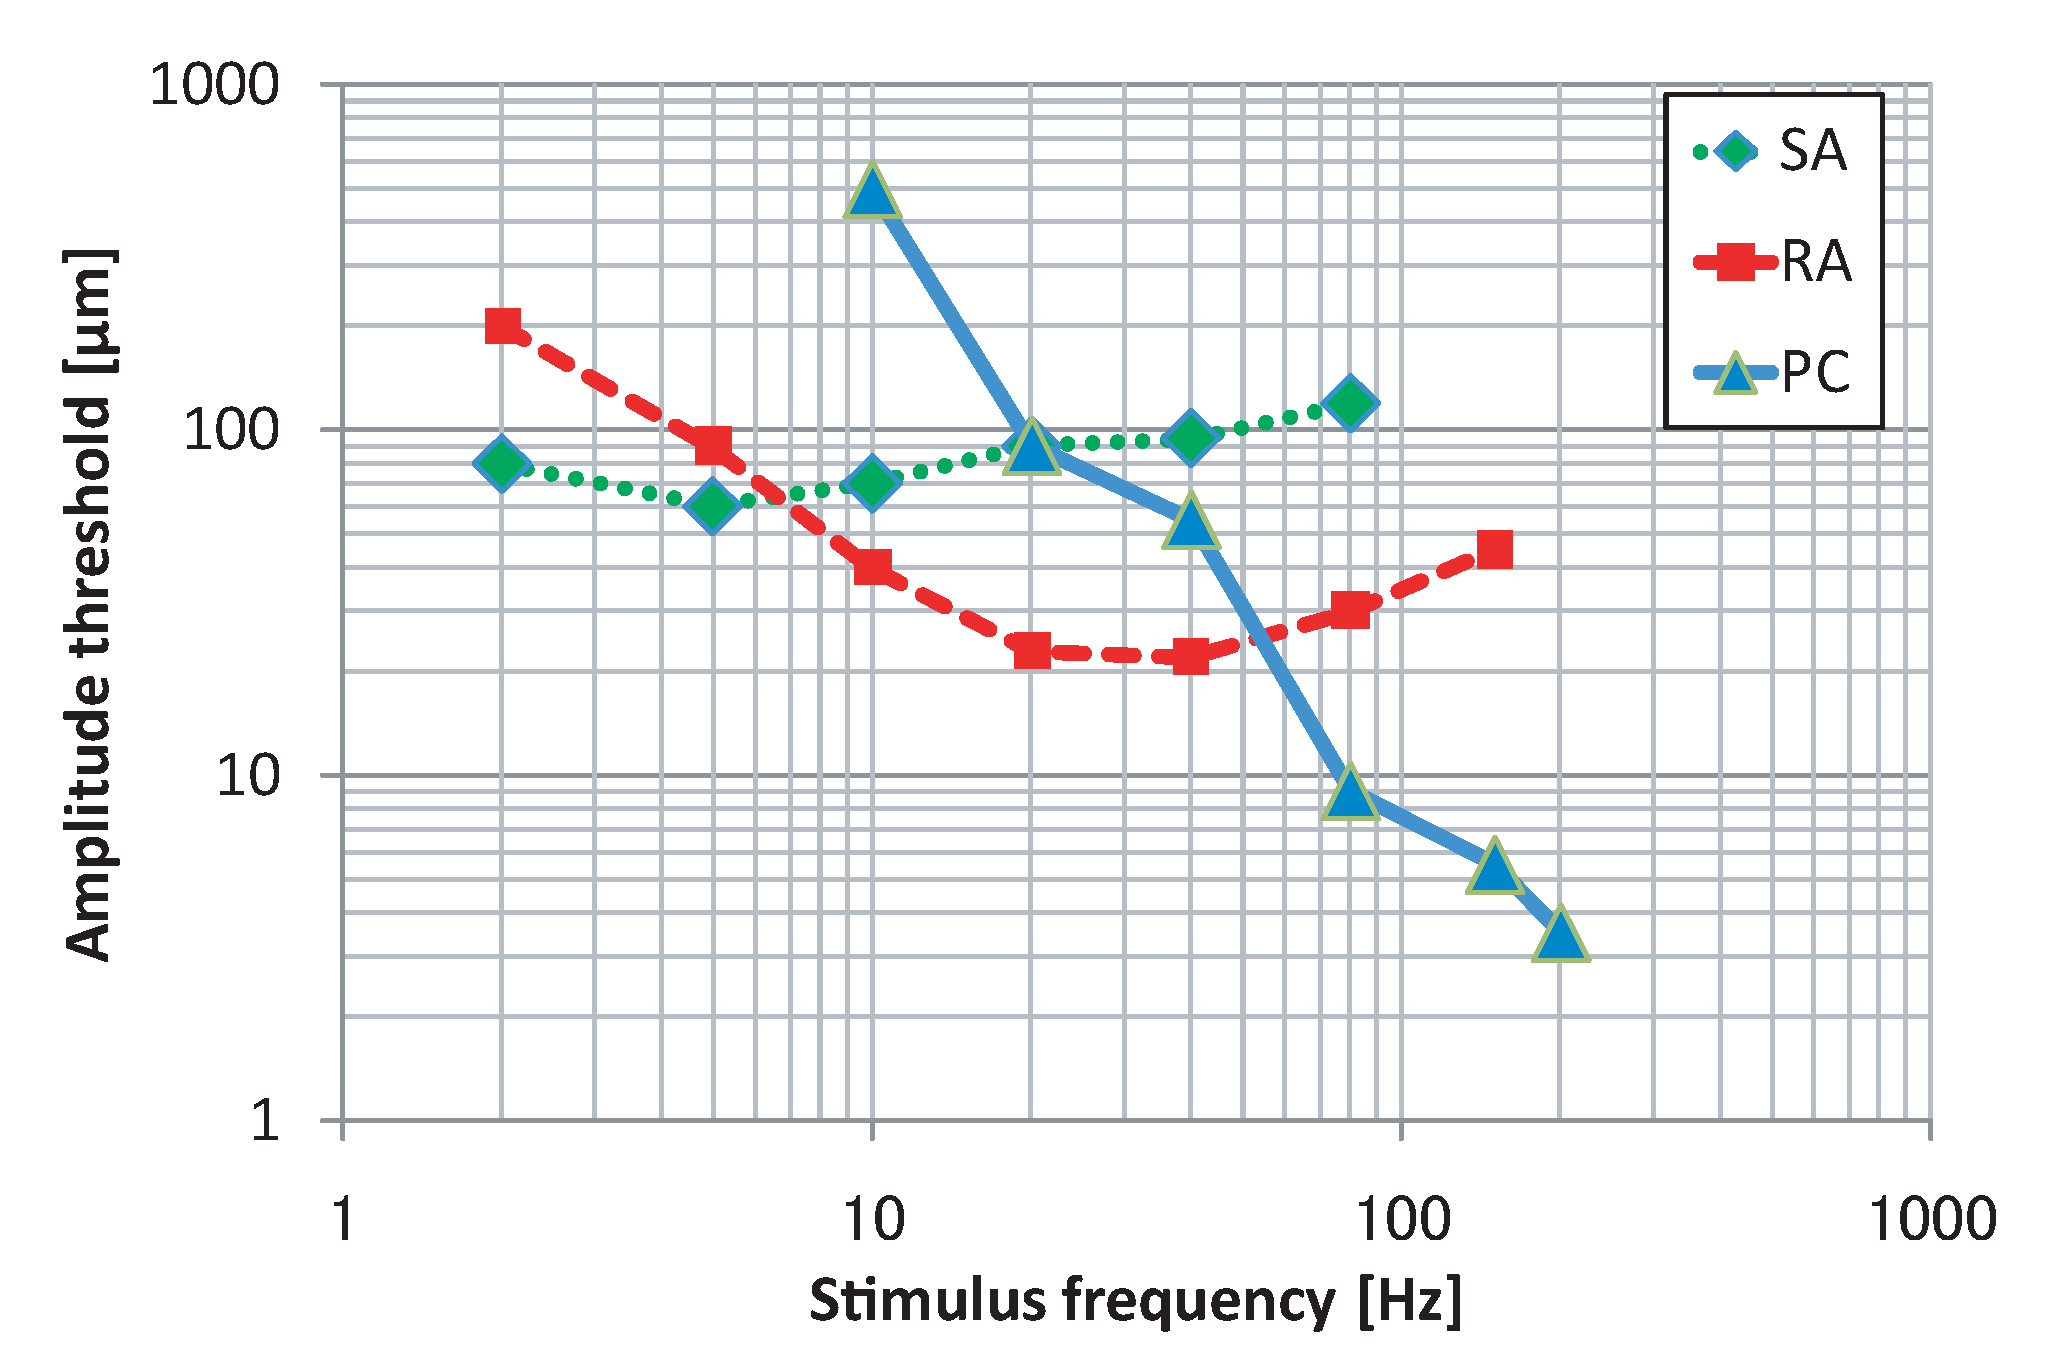
\includegraphics[width=14cm]{SARAPC.eps}
   \caption{時間周波数特性(\cite{Freeman:1982:Response}より改変)}
   \label{2-2}
  \end{center}
 %\end{minipage}
\end{figure}

\subsection{空間周波数特性}
正弦波などの周期的パターンが単位長当たり繰り返される回数を空間周波数といい,
信号の伝達特性は空間周波数に応じて変化する.この特性を空間周波数特性という.

\newpage

\section{剪断力}
本論文における剪断力とは,指を平面などに押し付けたときに,
押し付ける方向とは垂直な方向に働く力のことを指す.
例としては摩擦力などが該当する.
剪断力を用いた触覚提示の手法はMisnkyら\cite{minsky1990feeling}にはじまり,
多くの研究者によってなされている.
Sagaら\cite{saga2012lateral}は剪断力を用いることで
2.5次元的な形状提示を提案してきた.
本研究はこの剪断力を用いた錯覚に基づくものである.

\section{剪断力提示装置}
剪断力提示装置とは,Spidar Mouse\cite{五十嵐達郎:2010:SPIDAR-mouseの提案}
をもとにtablet上で二次元方向の剪断力を指先に提示可能にした装置である.
本装置は,タッチパネルの4隅にあるDCモータからのびる糸をタッチパネル中心のポインタで結び,
そのポインタに指を置いてタッチパネル上を動かすことで使用する.
4隅にあるDCモータが糸を巻き取る量を適切に制御することでポインタを振動させ,
タッチパネル平面の2次元方向に剪断力を提示する.
剪断力提示装置の写真を図\ref{2-3}に示す.

\begin{figure}[h]
\begin{center}
  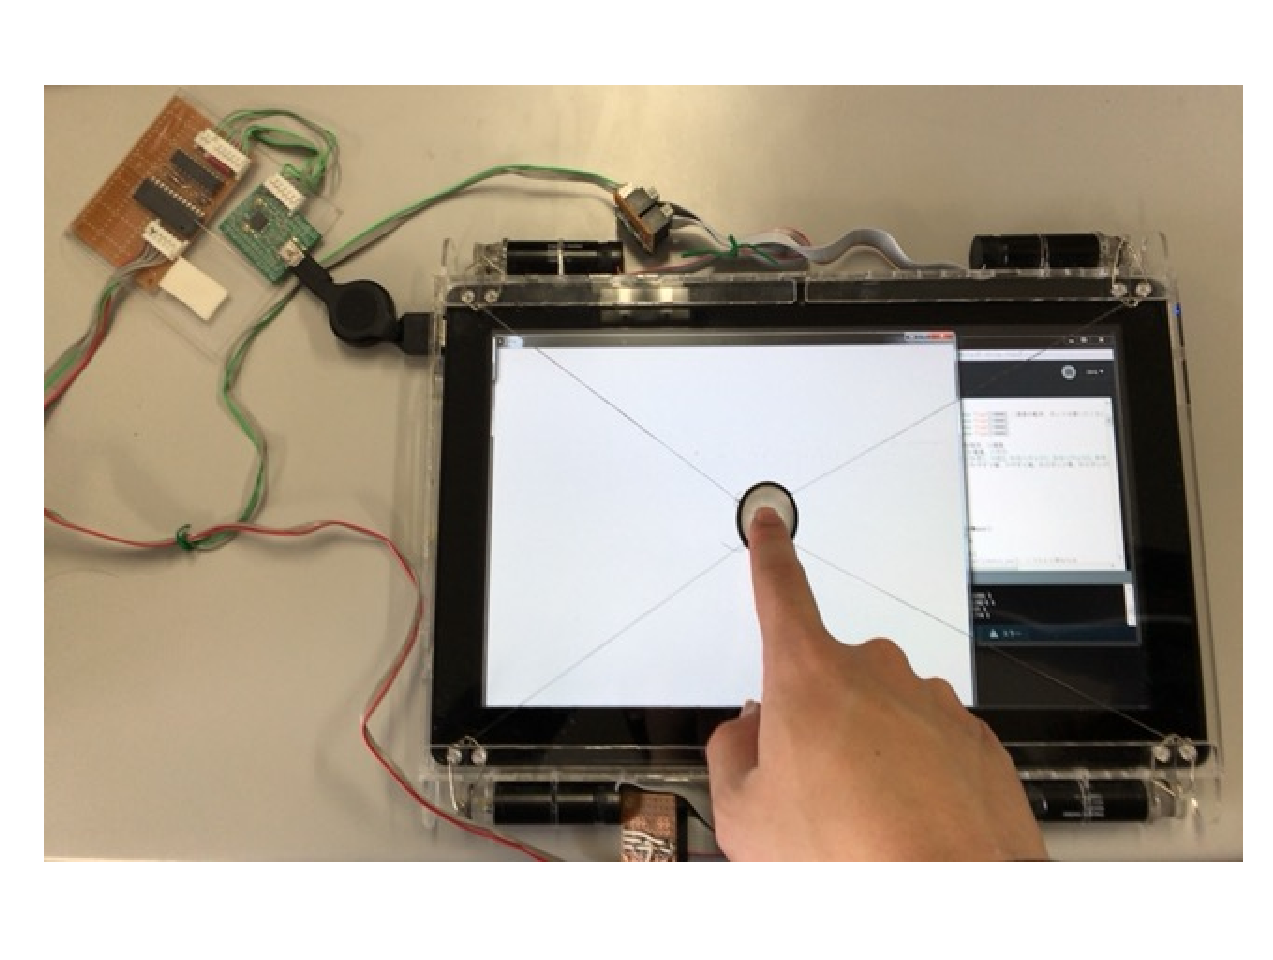
\includegraphics[width=15cm]{sptablet.eps}
  \caption{剪断力提示装置}
  \label{2-3}
\end{center}
\end{figure}

\section{振動情報を利用した触覚テクスチャ情報の提示}

\subsection{先行研究\label{2-4-1}}
振動情報を利用した触覚テクスチャ情報の提示手法として,
多くの研究者が様々な観点から研究を実施している.
Visellら\cite{visell2009toward}は床面での振動情報を記録,
再現することで,
新雪に踏み込んだような質感を再現している.
また,Minamizawaら\cite{minamizawa2012techtile}
はマイクや加速度センサの信号を増幅し,
ボイスコイルモータへの入力とすることで,さまざまな触感を再現している.
Romanら\cite{romano2012creating}はテクスチャを専用のツールで触察した
際の加速度,位置,時間の経過に伴う接触力の3つを記録し,それらを用いて
タブレット上にテクスチャを再現する手法を提案した.この手法では3次元の加速度を
知覚的に同等な1次元信号に変換し,
線形予測符号化を使用してこの触覚情報を周波数領域
の触覚モデルのデータベースに抽出している.そして,スタイラスを用いてタブレット上に
リアルタイムで記録した触覚情報をレンダリングすることで
仮想テクスチャを再現した.これらのアイディアをもとに,
KuchenbeckerらはVerroTouch\cite{VerroTouch}
という加速度を利用したテクスチャ情報提示手法を確立し,商用化している.
しかし,これらの研究では
様々な速度でツールを動かしたときの加速度や接触力を記録する必要があり,
1つのテクスチャの振動情報を記録するのに膨大な時間がかかるという問題がある.
また,ツールを用いて振動情報を記録,再現するため,
指で実際にテクスチャを触ったときの触覚を再現することは目標としていない.


Sagaら\cite{saga2013simultaneous}は接触力の測定を省略し,
振動の再現の際に補償手法を用いることで,
より簡単な記録/再生手法を提案している.
また,指で実際に触察したときの振動情報を3軸加速度センサで記録し,
記録した情報を剪断力提示装置を用いて再現することで,
スタイラスではできなかった実際に指で触ったときの触覚を再現している.

\subsection{記録振動の再現手法 \label{2-4-2}}
%\subsection{記録方法}
我々は,Sagaら\cite{saga2013simultaneous}の手法を拡張する形で,
X軸とY軸の振動情報を正確に記録,
これを我々のデバイスで再現する手法を提案する.比較のため,
本節ではSagaらにより提案されている補償手法を以下に記す.

\subsubsection*{補償手法}

記録時には加速度$a_{r}(t_{r})$と指の移動速度$\dot{x}_{r}(t_{r})$
が記録される.加速度$a_{r}(t_{r})$は音声入力の
サンプリング周期$f_{a}$ = 44.1\ kHzで記録されるため,
多くのデータ点を持つ.他方,指の速度$\dot{x}_{r}$,$\dot{x}_{p}$は
タッチパネルのサンプリング周期$f_{s} \simeq$\ 20 Hzで記録されるため,
加速度情報よりデータ点数が少ない.さらにモータによる振動信号の制御周期$f_{v}$は
$f_{v} <$ 10\ kHzとなっている.このそれぞれの周期$f_{a}$,$f_{s}$,$f_{v}$
の違い,また記録時と再生時の指の速度の違いを補償するため次式を導入し,正確なタイマ
を用いることで周期$f_{v}$に即した出力を得る.ここで,記録/再生時のフレーム間
時間差は$\Delta t_{r} \simeq \frac{1}{f_{a}}$,
$\Delta t_{p} \simeq \frac{1}{f_{v}}$である.添字のr,pはそれぞれ
記録/再生時を表す.式4より,指の記録/再生時の移動速度$\dot{x}_{r}$,
$\dot{x}_{p}$の比を利用して,記録振動振動から信号を再サンプリングする.\par
\begin{eqnarray}
t_{r_{n+1}} &=& t_{r_n} + \Delta t_r \\
t_{p_{n+1}} &=& t_{p_{n}} + \Delta t_{p} \\
a_p(t_{p_{n+1}}) &=& a_r(t_{p_{n}} + \frac{|\dot{x}_p(t_{p_{n}})|}
{|\dot{x}_p(t_{r_{n}})|} \cdot \Delta t_{p} )
\end{eqnarray}

位置情報ではなく速度情報の比と正確な時間情報を併用することにより,それぞれ
の周期$f_{a}$,$f_{s}$,$f_{v}$の違いを補償している.
この手法により多くのテクスチャ情報が簡単なサンプリングにより
提示可能になる.しかしながら,記録情報には接触力に関する情報がないため,
生成される振動の再現性は低くなる.\par

\subsubsection*{振動方向}

また,それまでの既存研究における振動を用いたテクスチャ表示は,
振動子としてボイスコイルなどを利用することが多く,振動方向が固定であった.
そのため,振動方向によるテクスチャ再現性の効果を検証できなかった.
剪断力提示装置は糸の張力による2次元での力の提示が可能であるため,
パネル平面の2次元上での振動方向制御が可能である.
Sagaら\cite{saga2013simultaneous}は振動方向によるテクスチャ再現性
の検証もおこなっている.指の動きに平行な接線振動$(F_T)$と,指の動きに垂直かつ
タッチスクリーン面に平行な陪法線振動$(F_B)$
の2方向の振動のどちらがテクスチャ提示に適切であるのか,
心理物理実験を通じて検証した.2方向の振動を図\ref{3-2}に示す.


\begin{figure}[t]
\begin{center}
  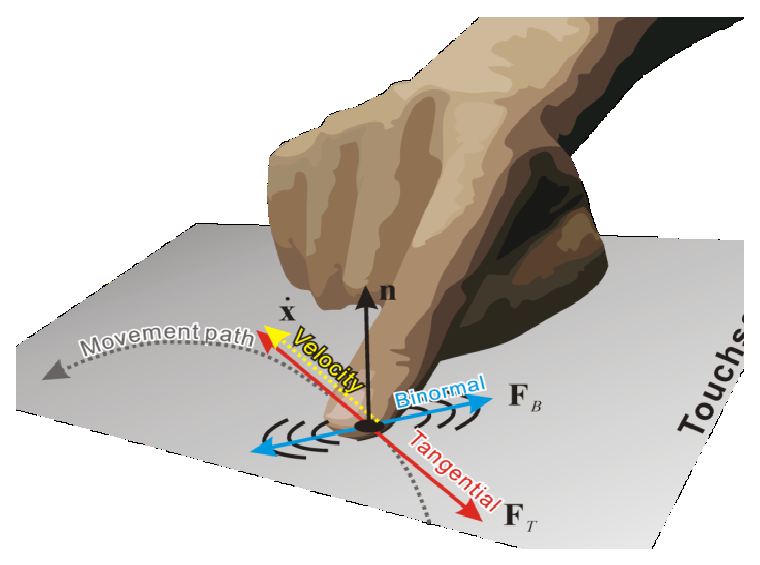
\includegraphics[width=11.0cm]{sinndou.eps}
  \caption{振動方向}
  \label{3-2}
\end{center}
\end{figure}

紙やすり,製氷皿,カーペット2種,スポンジ2種,柄タイル,鉄やすり
の8種類のテクスチャを用いて実験を行った結果,以下の内容が分かった.
\begin{itemize}
  \item カーペットや研磨スポンジといった柔らかい素材においては$F_S$が適している
  \item 柄タイルや製氷皿といった硬い素材においては両手法に有意な差はない
  \item 紙やすりといった硬い素材だがランダムな空間周波数をもつものにおいては
  $F_B$が適している.
\end{itemize}
この研究は振動方向がテクスチャの再現性に与える影響を検証しており,
仮想テクスチャを再現する上での1つの指標になる.
しかし,この研究では2方向の振動のみを検証しており,記録された振動をそのまま
再現する試みは行われていない.本研究ではこれらの研究を参考にし,記録した振動
のX軸とY軸を正確に再現するアルゴリズムの実装と
剪断力提示装置を用いて提示したときの再現性の検証を行う.


% Local Variables:
% TeX-master: "main"
% mode: yatex
% End:
